\chapter{以密码之剑护网安之城}
\label{cha:introduction-to-cryptology}

\begin{intro}
  在网络越来越发达的今天,网络安全早已成为国家安全的头等大事之一。但这份「安全」,要靠人类不断发展与精进的密码学来守护。这一章,我们来走进密码学的世界,探寻数字与文字间的舞蹈,以及密码如何守护网络世界的安全。读完本章,你应该有了下面这些问题的答案:
  \begin{itemize}
    \item 为什么网络世界中危机四伏?
    \item 什么是「密码」,它和我们平常使用的「登录密码」有何联系?
    \item 从古至今,世上有哪些有代表性的密码?
    \item 「HTTPS」是什么?为什么有时浏览器会提示「网站不安全」?
    \item 当今的密码如何保证我们的信息在网络中完整与安全?
  \end{itemize}
\end{intro}

今天的世界已经离不开网络,从我们的日常生活到政府各项事务的管理,从企业的高效运转到顶尖的科学技术,网络已经成为了这一切的基石。可是你是否想过,这个网络世界其实危机四伏?我们在网络上传输的信息,可以很轻易地被窥探、拦截和篡改;企业与企业、国与国之间,网络已经成为没有硝烟的战场。这样的环境之下,密码学技术帮助人们保护信息的安全,而以密码学为武器,人们构建起了「网络安全之城」,进而造就了今天绚丽多彩的网络世界。

\section{危机四伏的网络世界}

网络世界之所以危机四伏,从某种意义上来说,和当今互联网的底层技术——「分组交换」——脱不了干系。

我们说网络连接了世界的每一个角落,但这么多角落都依靠「点对点」的直接连接显然不太现实。事实上,网络之所以称为「网络」,正是因为它如同我们不时见到的蜘蛛网一样,由许多「结点」张成,信息在结点之间「转发」,形成一条虚拟的「通路」。

为了提升信息在结点之间传输的效率,网络会将我们需要发送的数据切成许多一定长度的小片段,这些片段就像一个个快递包裹一样,流入一个个结点。每个结点如同快递的转运中心,根据片段上标记的「目的地」信息,将片段转发给去往目的地的下一个结点。就这样,经过一次次转发,我们的数据片段都会抵达终点,并重新组装为完整数据。这种传输方式称为「分组交换」,它奠定了互联网的传输基础。

\begin{figure}[htb!]
  \centering
  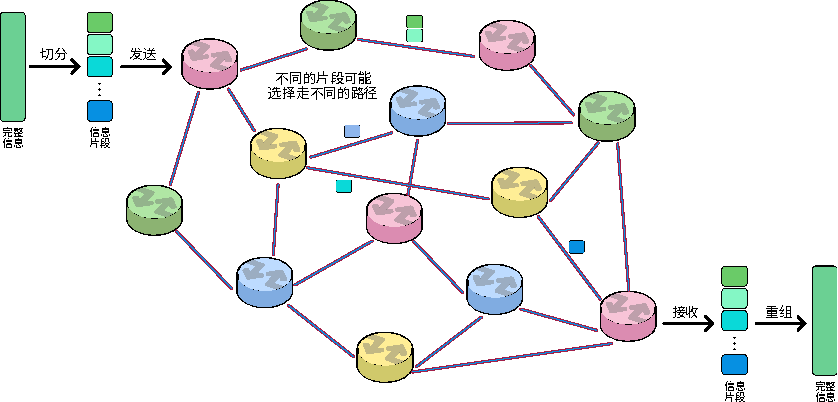
\includegraphics[width=.9\textwidth]{assets/surpass/Packet_routing.pdf}
  \caption{基于分组交换的网络}
  \label{fig:Packet_routing}
\end{figure}

然而,看似十分完美的过程,实际上充满危机。在网络上传输的数据可以很轻易地被截获,甚至直接修改也不是什么难事:攻击者只要攻击、控制了网络中的一个结点,所有经过它的数据片段都一览无余。如此一来,攻击者可以随意篡改数据片段的内容,或者将数据拦下,让目的地收到不完整的信息。攻击者甚至可以用我们的名义发送伪造的信息,从而造成具有破坏性的后果。

如果我们能将数据加密,使得加密后的信息即使被截获,攻击者也无法得知其中内容,就能在一定程度上解决这个问题。若是还可以设计出校验信息完整性、真实性的方法,传输的安全性又能再跃上一个台阶。随着密码技术的发展,这一切都渐渐成为了可能——接下来,让我们推开密码世界的大门,领略今天的「密码之剑」如何铸成。

\section{蓬勃发展的密码学}

\subsection{人类的「传统艺能」}

{
  \centering\vspace*{-4pt}
  \fontsize{5pt}{6pt}\selectfont\color{black!10!white}
  S\hspace{\fill}t\hspace{\fill}e\hspace{\fill}g\hspace{\fill}a\hspace{\fill}n\hspace{\fill}o\hspace{\fill}g\hspace{\fill}r\hspace{\fill}a\hspace{\fill}p\hspace{\fill}h\hspace{\fill}y\par
  \vspace*{-4pt}
}

几千年来,「如何让信息保密」这个问题一直伴随在人类文明左右:从古代战场间的传令、军中机要情报的转移、能工巧匠家里的祖传秘方,到如今网络世界的信息流转……种种危机四伏的场景,如何让这些重要信息不被闲杂人等知晓?「隐写术」和「密码学」,就此成为了人类的「传统艺能」。

「隐写术」(steganography),顾名思义,就是把重要信息「隐藏着写下来」,让读它的人基本不会注意到重要信息的手段。虽然它不算一种密码,但在「使信息对不知道的人来说很难看出来」这方面,它和密码是一样的。

古罗马的古典诗人奥维德就曾记录过用新鲜牛奶写信的隐写术——这样写在纸上的字很快会消失不见,但是如果点燃字迹的一角,就可以将字迹显现出来。除了牛奶外,一些植物汁液、明矾、果汁等也被用作隐形墨水。除此之外,有人将信息写在树叶上、衣服里或是身体上,再想办法进行遮掩;还有人使用「藏头诗」来隐匿信息……可是,只要隐藏的信息被看见,外人仍能读懂它,这也是隐写术的特点——明文隐写。

\begin{note}
  在现代,为了解谜游戏的谜题,或为了实现某些特殊的效果,隐写术焕发了第二春。譬如本节的开头就藏着小小的一行「Steganography」。
\end{note}

与隐写术相比,密码学(cryptography)的目标,则是将内容变换成常人看不懂的模样,这样的技术称为「密码」(cipher)。公元前 5 世纪,古斯巴达人使用过一种叫做「密码棒」(Scytale)的器械:一根缠绕有羊皮纸条的木棍。人们把信息竖着写在羊皮纸条上,写完后取下纸条,字母顺序就被打乱,难以再看出原本的信息。需要阅读时,只需取一根同样规格的木棍,将纸条重新缠绕即可。这是人类历史上已知的最早的密码器械。

\begin{figure}[htb!]
  \centering
  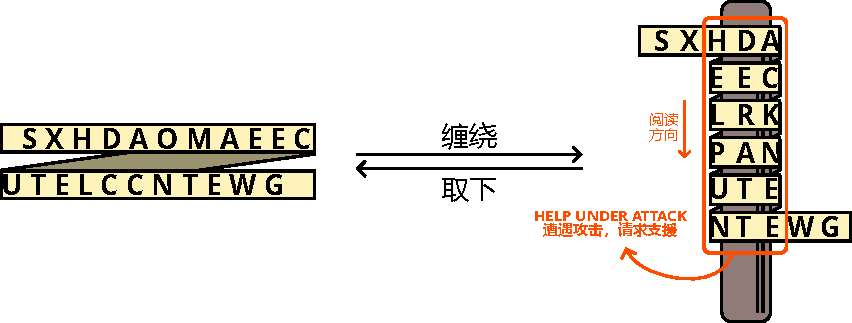
\includegraphics[width=.95\textwidth]{assets/surpass/Scytale.pdf}
  \caption{密码棒}
  \label{fig:Scytale}
\end{figure}

\begin{note}
  这里「密码」一词指的是将信息进行变换以进行保密的技术。而我们在生活中经常说的「登录密码」「开机密码」,虽然也叫「密码」,但是含义并不相同,\regcolor{它们的学名叫「口令」}。
\end{note}

古罗马的凯撒大帝使用过这种方法来保护重要的军事信息:将每个字母向后移动 3 位。如下图所示,左侧是一个加密轮盘,外圈和内圈上刻有一一对应的字母。当前内圈转到「3」的位置,我们可以利用它轻松地完成情报中字母的替换。

\begin{figure}[htb!]
  \centering
  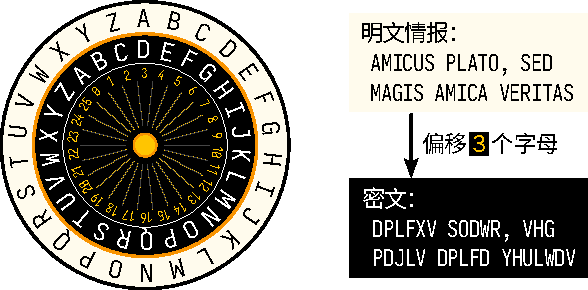
\includegraphics[width=.75\textwidth]{assets/surpass/CaesarCipher.pdf}
  \caption{凯撒密码}
  \label{fig:CaesarCipher}
\end{figure}

外人若不知道这种方法的具体细节——甚至,只要不知道具体的偏移量,外人就很难猜出原本的内容。这种密码被称为「凯撒密码」。事实上,凯撒密码不止局限于「3」这一个偏移量:通过旋转内圈到不同位置,我们就能使用 0 至 25 的不同偏移量。

\begin{note}
  所以任何一段正常的英文文本都是偏移量为 0 的凯撒密码密文。
\end{note}

在这些例子中,原始信息称为「明文」,经过处理后,难以理解的信息称为「密文」。将明文转换为密文的过程称为「加密」,而反过来就是「解密」。为了完成这两个过程,我们需要用到额外信息——「密钥」,它就像一把钥匙,加密与解密都是需要它来打开的门扉。例如,对于密码棒来说,密钥是密码棒的尺寸;对于凯撒密码,密钥就是它的偏移量——3 这个数字。

然而,凯撒密码非常容易破解。偏移量只有 26 种情况,一个个试都能试出正确的密钥。于是,人们随后发明了「字母替换密码」:直接重排字母表,将每个字母替换成另一个字母。例如:

\begin{table}[htb!]
  \centering
  \caption{一种字母替换密码表}
  \label{tab:replace-alphabets}
  \begin{tblr}{
    cells = {halign = c, font = \ttfamily},
    column{1} = {halign = c, fg = white, bg = missing, font = \bfseries},
    column{even} = {MissingSkyBlue},
    colsep = 4pt,
  }
    \toprule
    原文 & A & B & C & D & E & F & G & H & I & J & K & L & M & N & O & P & Q & R & S & T & U & V & W & X & Y & Z \\
    密文 & Q & W & E & R & T & Y & U & I & O & P & A & S & D & F & G & H & J & K & L & Z & X & C & V & B & N & M \\
    \bottomrule
  \end{tblr}
\end{table}

这样一来,「MISSING」一词加密之后就变成了「DOLLOFU」。相比凯撒密码,字母替换密码更隐藏了字母之间的相对位置关系,而高达$26!$种加密情况也使得它更难被暴力破解。可是,人们在统计了大量文本后发现,一门语言当中,每个字母出现的频率是有规律的:譬如 E 与 T 是在英语中出现频率最大的两个字母。那么,密文里出现频率最高的两个字母,就很可能对应着 E 和 T。这就是「频率分析」。借助它,人们可以确定字母间的对应关系,从而破解字母替换密码。

采用「动态替换」的维吉尼亚密码则在一定程度上解决了这个问题。它使用一个单词作为密钥,靠密钥的每个字母决定不同位置的偏移量:例如 B 代表偏移量为 1,D 就代表偏移量为 3。下图展示了用「WINDY」加密「MISSING」的过程,可见,每一次的偏移量都在变化,并且不同位置上,字母的替换关系不同。

\begin{figure}[htb!]
  \centering
  \includegraphics[width=.47\textwidth]{assets/surpass/VigenèreCipher.pdf}
  \caption{维吉尼亚密码}
  \label{fig:VigenèreCipher}
\end{figure}

密码学伴随着人们保密意识的产生而诞生,然而直到 20 世纪 50 年代,密码学的本质都没有什么变化。各种加密方式都可以归类为「代换」和「置换」两种变换的组合:代换指的是「用一种字母替代另一种字母」,而置换指的是「变更不同字母的位置」。上文提到的密码棒就是一种置换密码,而凯撒密码及其衍生版本则是代换密码。

在这一时期,密码的安全性,来源于代换和置换的精巧设计;而这样的设计,或基于经验,或基于直觉。因此,此时的密码学是一门「艺术」——比起严格的论证,它更侧重人类头脑中的灵光一闪。如今,我们把这整个时期的密码学都称为「古典密码学」,而相关的密码则称为「古典密码」。

1949 年,美国数学家、工程师香农的《保密系统通信理论》(\textit{Communication Theory of Secrecy Systems})从数学和信息论的角度阐明了关于密码系统的分析、评价和设计的科学思想,提出了有关密码学的完整数学模型。这篇论文用数学的语言,定量地描述了密码的「安全性」,以及与其相关的一系列概念,如密钥的复杂度、加密的复杂性等等。它让密码从一门基于感性构造、精巧设计的艺术,开始走向基于理论分析、实验验证的科学。

自此,密码学的发展有了理论的指导,近代密码学的序幕就此拉开。

\subsection{对称密码的发展}

\subsubsection{一把钥匙开一把锁}

第二次世界大战期间,纳粹德国使用一种被称为「恩尼格玛」(Enigma,意为「谜」)的密码机来加密军事通讯。它形如一台打字机,但不能在纸上打字;相反,它有一个由 26 盏小灯泡组成的显示板,排布如键盘一般。此外,在机器上方,它还装有几个印有字母的机械转盘(称为转子)。下方左侧就是一种常见型号的恩尼格玛密码机的示意图。当使用者在键盘上击键时,某个不同字母\footnote{没错,这正是恩尼格玛密码机的特点之一:加密后的字母绝不与原始字母相同。你可以在阅读下面的介绍后思考一下这是为什么。}对应的小灯就会亮起——这便是对应字母加密后的密文。

\begin{figure}[htb!]
  \centering
  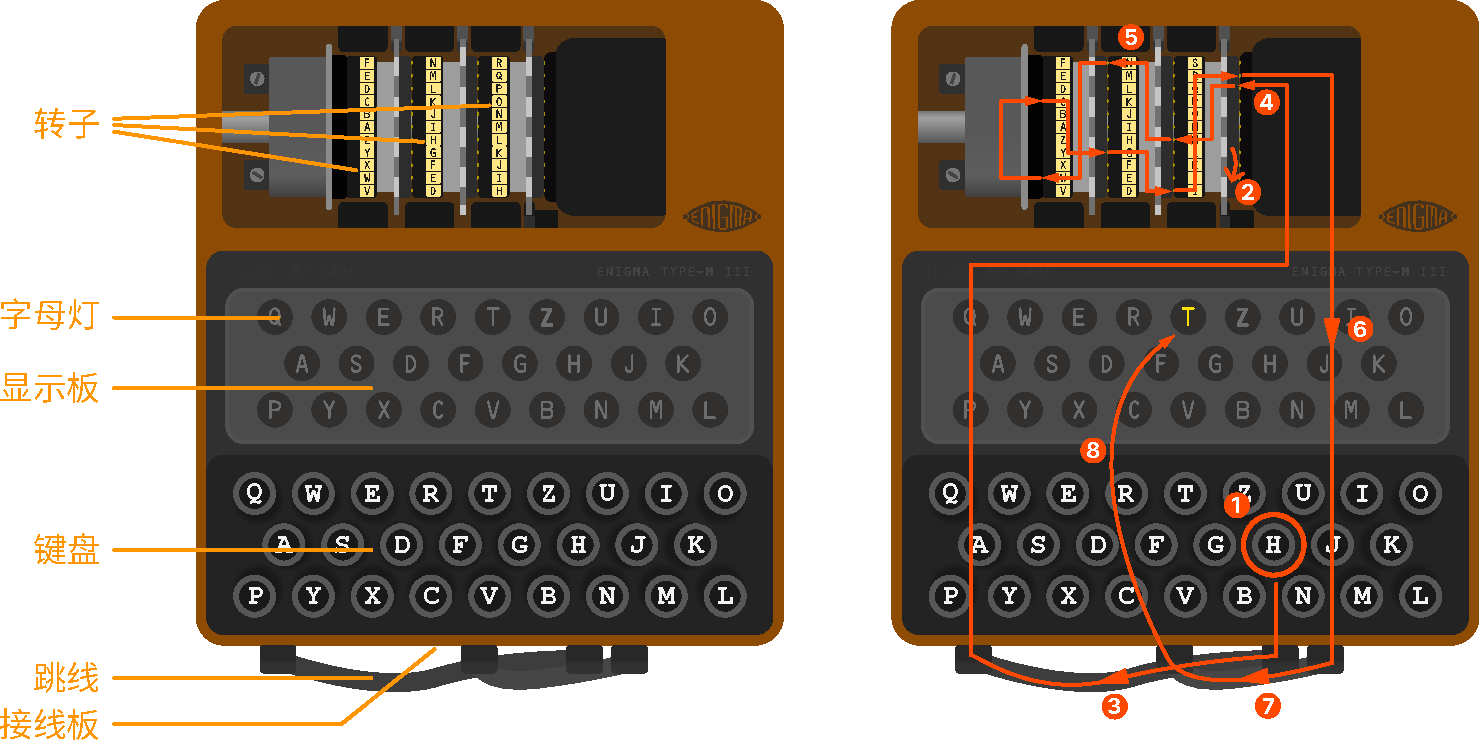
\includegraphics[width=.9\textwidth]{assets/surpass/Enigma.pdf}
  \caption{恩尼格玛密码机}
  \label{fig:Enigma}
\end{figure}

上方右图展示了恩尼格玛密码机大致的工作原理。每 \CJKunderline{➊ 按下一个键},\CJKunderline{➋ 转子就转动一格}。转子之间有联动机构——当一个转子转完一圈后,它左边的转子也会转一格。同时,按下的键发出一个电信号,并首先被传到「接线板」,在这里分布着对接到不同字母的插孔,使用者可以 \CJKunderline{➌ 插上一些「跳线」,将信号在连接的字母间对换}。紧接着,\CJKunderline{➍ 电信号进入第一个转子}。不同的转子内部会按各自的规则替换字母,使用者可以按需选用不同型号的转子。\CJKunderline{➎ 信号依次流过三个转子,并在折返后再反向流回去。}此时,电信号代表的字母已经和原来按下的字母相去甚远了。最后,\CJKunderline{➏ 信号再被送入接线板}进行 \CJKunderline{➐ 最后一次替换},然后 \CJKunderline{➑ 点亮对应字母的灯泡}。

\begin{note}
  上节介绍了「明文」「密文」「密钥」的概念,那么恩尼格玛密码机的明文、密文和密钥是什么?
\end{note}

在这样的一整个流程中,字母一共经过了 8 次替换,而且由于转子随每次击键而旋转,这种替换关系每输入一个字母就会变化,使得字母之间的对应关系变得极其复杂,最终的密文与原文看起来毫无联系。但解密却很简单,只需要在另一台相同型号的密码机上安装相同的转盘,调整到相同的起始位置,并以相同方式连接跳线,输入密文,即可打出原始的明文。

二战前期,德军在战场上节节胜利,一定程度上依靠了恩尼格玛密码机强力的加密效果,让他们顺利隐藏自己的情报与动向。同时,盟军则为破解恩尼格玛密码机付出了不少努力:早在 20 世纪 20 年代,德国已经开始使用恩尼格玛密码机。1927 年,英国方面买了一台商用恩尼格玛密码机,花了十年终于成功破解,但可惜没法用在军用机上。而同期波兰的研究者依靠对德语的了解与一些间谍活动,初步破解了三转子的军用密码机。二战期间,盟军基于这些成果,外加德军的一些疏漏,才成功破解恩尼格玛密码机,并逐步扭转战局。

\begin{note}
  据说在热门网络游戏《第五人格》中,玩家需要破译的「密码机」,设计原型就是恩尼格玛密码机。
\end{note}

无论是凯撒密码还是恩尼格玛密码机,它们都有一个共同的特征:\regcolor{加密和解密过程使用相同的密钥}。解密凯撒密码,只需加密时使用的偏移量即可;而对于恩尼格玛密码机,则需要知道加密时使用的转子型号、转子起始位置以及跳线连接情况。\regcolor{这样的密码被称为「对称密码」},如同现实生活中的钥匙和锁,用相同的钥匙来上锁和开锁。对称密码是最基本的一种密码形式,它符合我们对「加密」这件事的直觉,因此当密码学从古典时期迈向近代时,人们首先研究的,便是如何设计出安全、高效的对称密码。

\subsubsection{混淆与扩散}

前文我们提到,古典密码的设计模式,总可以分成代换和置换两类。前者替换内容,后者更改位置。在近代密码学中,人们从信息论的角度对这两类方式进行了概括和发展,代换与置换法随之进化为「混淆」和「扩散」。

\begin{itemize}
  \item 「混淆」旨在掩盖密文和明文之间的对应关系,最简单的方式是代换。增强混淆效果则需要设计更加复杂的变换方式。恩尼格玛密码机通过多个旋转转盘改变字母映射,其实亦是一种混淆。
  \item 「扩散」的目的是将单个字母加密所带来的影响扩大——譬如,加密一个字母,可能会改变密文中多个字母的表示。置换是扩散的最简单方式,但能力非常有限——只能影响某处单单一个字母。而现如今使用的各种对称加密算法,都能做到「原文改变一点点,密文改变一大片」。
\end{itemize}

优秀的密码算法,就是科学地结合混淆和扩散,实现最大的安全性。顺着这样的思路,我们介绍两款在密码学历史上具有重要意义的对称加密算法:曾经风光无限但已寿终正寝的 DES,以及今天正在广泛使用的 AES。

\subsubsection{数据加密标准(DES)}

20 世纪 70 年代,随着美国政府开始重视计算机安全问题,美国国家标准局(NBS,现为美国国家标准与技术研究院 NIST)开始征集用于政府内信息加密的算法。最终,IBM 公司提出的一套算法得到采用,NBS 为它赋予「\regcolor{数据加密标准}」(Data Encryption Standard,\regcolor{简称 DES})的名字并正式公布。DES 算法采用了一种「分组加密」的思路——将明文先切割成固定 64 位长的块,再逐块加密,块与块之间的加密可以互相影响,这些块的密文最终合成为一条完整的密文。解密时,只需反向切割密文,再逐块解密即可。

\begin{note}
  在本章后续的介绍中,「位」均指「二进制位」,比如「64 位的明文」指明文由 64 位二进制数(即「比特(bit)」)组成。
\end{note}

DES 对每一块加密时,都会使用 56 位长度的密钥来\regcolor{循环进行 16 次包含代换和置换的操作}。其中的代换部分,DES 使用一套预先设计好的代换表——「S 盒」施行。下表就是其中一个 S 盒。对于十六进制数据 \MissingTT{2E},寻找第 \MissingTT{2} 行第 \MissingTT{E} 列的值,就能得到代换后的结果 \MissingTT{B},即 11。DES 一共有 8 个这样的 S 盒,它们互不相同,每个都是经过特定设计得到的,可以在加密过程中引入复杂性来防止被轻易破解。

\begin{table}[htb!]
  \centering
  \caption{DES 的一个 S 盒}
  \label{tab:DES-s-box}
  \begin{tblr}{
    hline{2} = {2-Z}{solid,white},
    vline{2} = {2-Z}{solid,white},
    hline{2-Y} = {1}{solid,white},
    vline{2-Y} = {1}{solid,white},
    hline{3-Y} = {2-Z}{solid,missing},
    vline{3-Y} = {2-Z}{solid,missing},
    hline{1,Z} = {solid,missing},
    vline{1,Z} = {solid,missing},
    columns     = {c},
    colsep      = 1pt,
    row{1}    = {font=\ttfamily\bfseries, bg=missing, fg=white},
    column{1} = {font=\ttfamily\bfseries, bg=missing, fg=white, wd=3em},
    column{2-Z} = {2em},
    cell{1}{1} = {bg=MissingSkyBlue, fg=missing},
  }
    \diagbox[width=3em]{行}{列} & 0 & 1 & 2 & 3 & 4 & 5 & 6 & 7 & 8 & 9 & A & B & C & D & E & F \\
    0\_ & E & 0 & 4 & F & D & 7 & 1 & 4 & 2 & E & F & 2 & B & D & 8 & 1 \\
    1\_ & 3 & A & A & 6 & 6 & C & C & B & 5 & 9 & 9 & 5 & 0 & 3 & 7 & 8 \\
    2\_ & 4 & F & 1 & C & E & 8 & 8 & 2 & D & 4 & 6 & 9 & 2 & 1 & B & 7 \\
    3\_ & F & 5 & C & B & 9 & 3 & 7 & E & 3 & A & A & 0 & 5 & 6 & 0 & D \\
  \end{tblr}
\end{table}

\begin{note}
  想知道 DES 的具体过程?受限于篇幅和本文的定位,我们在此处不作过多介绍,你可以自己上网搜索。
\end{note}

1975 年,DES 正式对外公布,并在 1976 年被定为美国联邦标准。DES 的提出,在密码学历史上具有里程碑式的意义。DES 公开后,没过几年就成为了世界上使用最为广泛的加密算法:政府、企业、民间都开始使用 DES 保护重要数据。另一方面,DES 所使用的分组加密思想、费斯妥结构和密钥扩展等思路,启发着无数后继加密算法的研究。

然而,有关 DES 算法本身的争论从它诞生开始就没有停息。围绕 DES 算法本身,争论的焦点有两个,其一便是 \regcolor{56 位的密钥是否足够安全}。任何密码都存在通过穷举所有可能的密钥来破解的可能,这就是「暴力破解」。而实际破解的难度会随着算力的发展快速下降:在 1977 年,就有学者构想了一台造价 2000 万美元,可以在 1 天内暴力破解 DES 密码的机器。到了 1993 年,同类机器的理论成本降到了 100 万美元,时间缩短到 7 小时。而在 1998 年,一台造价只有 25 万美元的破解机器被实际造出,从此破解 DES 成为事实上的可能。除了暴力破解外,一系列更高效的破解算法亦于上世纪末出现,它们让 DES 从「安全无比」的神坛上跌落,向人们昭示着密钥长度的重要性。

而有关 DES 的另一个争论,便是其神秘的 S 盒设计。我们刚才提到,DES 一共使用了 8 个 S 盒执行代换,而它们是人为设计并公开给大众使用的——那么,为什么这些 S 盒要这样设计呢?它们是否真的足够「安全」?尽管 S 盒的设计声称安全无比,并能防御多种破解方式,但是这些设计\regcolor{是否存在不为人知的甚至是刻意留下的漏洞}呢?由于 IBM 并没有完全公开 S 盒的设计方法,这些问题变成了悬在人们头上的利剑,而执剑人则隐藏在黑暗之中。人们开始思考,能否让 S 盒的构造方式变得透明,同时仍然保持足够的安全。

基于各种安全原因,1999 年,DES 被要求「只能在遗留系统中使用」,新的系统必须使用 DES 的升级版——三重 DES(Triple DES,简称 TDES 或 3DES),使用两个密钥进行 3 次 DES 加密。然而这只是「换汤不换药,治标不治本」罢了。2005 年,美国官方不再使用 3DES,但 3DES 依然是可选标准。2018 年,NIST「退役」3DES,从此 3DES 只能在老旧的系统中使用,各种软件纷纷开始移除对 3DES 的支持。

2023 年 6 月,NIST 发布公告,宣布将于 2024 年 1 月 1 日起,正式废止有关 3DES 的使用建议,这标志着美国完全抛弃 3DES。而各地的软件厂商亦已用更安全的加密算法完全替代它,属于 DES 的时代画上了句号,它的后继者——高级加密标准(Advanced Encryption Standard,简称 AES)则在今天继续守护着我们的安全。

\begin{figure}[htb!]
  \centering
  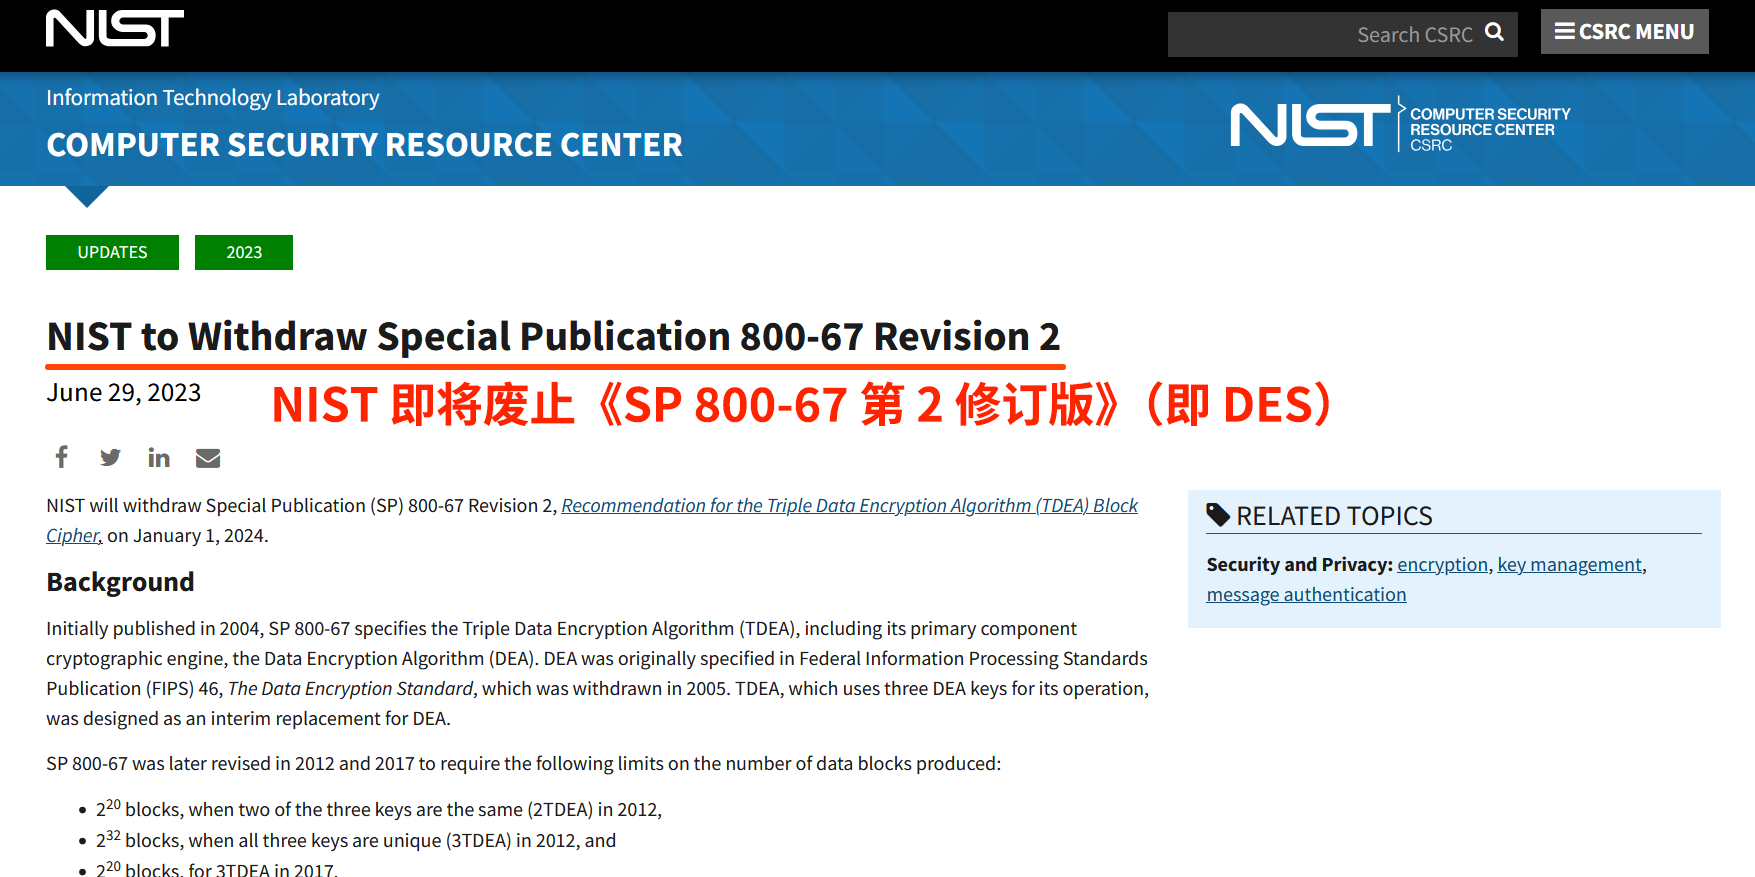
\includegraphics[width=.85\textwidth]{assets/surpass/NIST_announcement.png}
  \caption{NIST 退役 3DES 的公告}
  \label{fig:NIST_announcement}
\end{figure}

\subsubsection{高级加密标准(AES)}

在上世纪末 DES 被证明不再安全之际,人们除了「亡羊补牢」式地急忙提出 3DES 算法外,亦开始寻找新的更安全的加密算法。1997 年,NIST 开始为「\regcolor{高级加密标准}」(Advanced Encryption Standard,\regcolor{简称 AES})征集加密算法。在经过数年的甄选后,2001 年,由比利时密码学家 Joan Daemen 和 Vincent Rijmen 所设计的一款算法脱颖而出,成功拿下 AES 的名号。自此,DES 系列算法渐渐走向历史的坟茔,而 AES 直到今天仍然是最广泛使用的对称加密算法,并且依然有着无与伦比的安全性。

和 DES 一样,AES 也是一种分组密码,同样采用了代换置换结合的方式完成一轮加密操作,亦通过多次循环来确保安全性。不过,AES 使用的结构与 DES 有所不同,密钥长度也不一样:\regcolor{AES 分组长 128 位,可以选择 128 位、192 位和 256 位三种不同长度的密钥},远比 DES 的 56 位安全。同时,相比于 DES 的 S 盒采用的人工设计法,AES 使用一个神奇的数学方法来生成 S 盒,因此其安全性可以得到严谨证明,不存在刻意留下漏洞的空间。

\begin{note}
  AES 的 S 盒,本质是在有限域 $GF(2^8)$ 上对素多项式 $m(x) = x^8 + x^4 + x^3 + x + 1$ 求逆。
\end{note}

AES 优秀的算法设计使其一直保持着足够的安全性。直到今天,人们仍然没有发现破解 AES 的实用方法。自 2002 年 NIST 将 AES 订立为标准以来,AES 已经成为了最流行的对称加密算法,在我们的生活中几乎无处不在。例如,你正在浏览的《你缺计课》网站本身,利用了 HTTPS 技术(详见后文)传输到你的眼前,其间就依靠 AES 加密来保证安全;在我们的手机、电脑内部,操作系统亦大量使用 AES 来加密存储敏感数据,防止设备失窃后的隐私泄露。

\subsection{非对称密码的兴起}

\subsubsection{令人头疼的密钥交换}

对称密码的不断发展,让数字时代资料的保密成为了现实。然而,无论是 DES、3DES 还是 AES,这些对称密码在用于数据传输时都有一个问题:加密和解密用的密钥,如何安全地在双方之间共享呢?

或许你会说,只要提前将密钥发送给对方就行了。但是请别忘记,我们之所以要加密通信,正是因为通信环境不安全——\regcolor{提前将密钥发送给对方,就有可能造成非常严重的后果:我们的「钥匙」可能遭到恶意拦截、伪造甚至调包,让之后的一切加密都形同虚设。}能否通过安全的物理手段——比如,线下碰个面——来提前沟通密钥呢?某些情况下似乎可行,但如果双方是未曾谋面的陌生人,恐怕就不太方便了。如此一来,寻找一种\regcolor{不需要提前共享相同密钥,就能实现加密通信}的方式,成为了摆在我们面前的现实问题。

先想象一个场景:在交通不发达的古代,Hans 和 Windy 相隔千里。现在,Hans 要将一则非常重要的机密信息用鸡毛信的方式传递给 Windy。由于路途漫长,信件在传递过程中几易其手,很难保证不被好事之人窥探。为了保证信息的安全,他们想到了一个这样的方法:

\begin{itemize}
  \item 首先,Windy 制作一个带锁的信封。这种锁和我们日常生活中用的门锁类似,\regcolor{锁上后需要用钥匙打开,但是开锁后用力一扣就能锁住,无需钥匙}。
  \item 接着,Windy 先把这个信封上的锁打开,将信封寄给 Hans,但钥匙留在自己手上。
  \item Hans 收到信封之后,把需要寄出的机要信息装进信封,用力一扣——现在,信封被锁住,除了 Windy 以外的任何人都无法打开它了。
  \item 最后,Hans 把这个装好信件的上锁信封寄给 Windy。Windy 收到后,用自己手里的钥匙将信封打开,取出信息。
\end{itemize}

就像这样:

\begin{figure}[htb!]
  \centering
  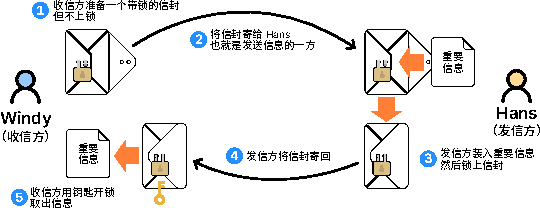
\includegraphics[width=.8\textwidth]{assets/surpass/Ancient_public_key_encryption.pdf}
  \caption{远古公钥加密}
  \label{fig:Ancient_public_key_encryption}
\end{figure}

在这样的过程中,\regcolor{通信双方之间并没有提前交换过任何「钥匙」},只要锁本身足够安全,就可以确保只有 Windy 自己能取出信件,而负责发信的 Hans 并不接触钥匙。当 Windy 要回复一则消息给 Hans 时,也只需先让 Hans 也做一个同类的信封,再走一遍相似的流程即可。

我们可以看到,在这不用提前交换钥匙就能实现双向保密的过程中,「带锁的信封」是关键,它有一个\regcolor{重要的「非对称」性质:上锁只需要用力扣上,而开锁需要使用钥匙}。将这个过程类比到加密、解密的过程,我们自然而然地想到——如果能设计一种\regcolor{加密和解密使用两把不同密钥的加密算法},不就可以完美地解决本节开头提到的那个问题了吗?

\begin{figure}[htb!]
  \centering
  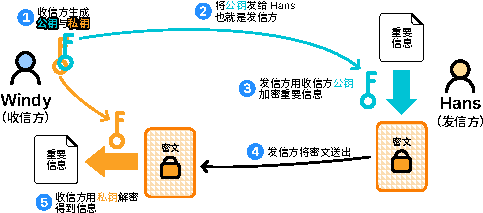
\includegraphics[width=.8\textwidth]{assets/surpass/Public_key_encryption.pdf}
  \caption{公钥加密}
  \label{fig:Public_key_encryption}
\end{figure}

不妨类比「带锁信封」来构想这样一种加密算法:\regcolor{为明文加密要使用密钥 P,但是解密密文则要使用密钥 S。}Hans 需要向 Windy 安全地发送一则消息,只需要先让 Windy 准备一对这样的 P 和 S。Windy 将 S 保留在手中,将 P 发送给 Hans——不必考虑安全与否,甚至直接将 P 公之于天下也行。Hans 看到后,将手中的消息使用 P 加密,再将密文直接发送给 Windy。现在,只有 S 能解开这则密文,而它始终留在 Windy 自己手里。信息被安全地传输,而用于解密的密钥全程未接触到外界。密钥 P 由 Windy 主动公开,我们称为「公钥」;密钥 S 始终留在 Windy 自己手里,我们称为「私钥」。公钥用于将明文加密成密文,而私钥用于解密。

Windy 持有的公钥和私钥,只能供别人给他发送消息,因此 Hans 也需要准备一对自己的公钥和私钥,并将自己的公钥公开出去。这样的加密方式就是「公钥密码」;又由于公钥、私钥的非对称性,也称「非对称密码」。这个系统看起来完美得不得了,只不过有一个小问题——这样神奇的加密算法真的能存在吗?还真别说,真就给人们找出来几个。

\subsubsection{单向函数、陷门与公钥加密}

先来做两个数学题:
\begin{enumerate}
  \item 计算 $97\times 47$ 的值;
  \item 已知两个质数 $p$ 和 $q$ 满足 $p\times q=4559$,求 $p$ 和 $q$。
\end{enumerate}

如果你真去算了两道题的结果,就会发现它们互为答案,并且各自是对方唯一的答案。然而,做这两道题的难度,则完全不在一个水平:第一题只需要简单的竖式乘法就能算出来,或许你还可以直接口算甚至心算;但对于第二题,如果没有第一题的铺垫,除了从 2 开始逐个尝试所有质数,似乎没有什么好方法了。可以想象,当 $p$ 和 $q$ 极其巨大时,就连计算机也很难解开问题 2。若将这样的运算视为函数,它们就是一种「单向函数」:「单向」说明它正着算很容易,倒着算很难。

现在,我们在问题 2 的基础上提供一点儿提示,让它变成如下的问题 3:
\begin{enumerate}
  \item[3.] 已知两个质数 $p$ 和 $q$ 满足 $p\times q=4559$,且 $p=97$,求 $q$。
\end{enumerate}
问题就变得十分简单,只需要进行一次除法运算,就能得到需要的结果。额外提供的提示($p=97$)并不是完整的答案,但在提供这个信息后,通向答案的路就从「山重水复疑无路」变成「柳暗花明又一村」了。像问题 2 这样「给点提示就能行」的单向函数称为「陷门函数」(trapdoor function),它们的反向计算过程仿佛在黑暗的地下室摸索前行,毫无头绪而极其困难;但如果用一些秘密信息,为我们提供一个「活板门」(trapdoor)出口,我们就能通过它爬出地下室,让计算顺利进行。

我们生活中常用的门锁也能算一个陷门函数。在开锁状态下,我们可以用力一扣就将它上锁——这如同陷门函数的正向过程。而如果使用蛮力,就很难将锁打开——这是陷门函数的反向过程。「钥匙」则是用来打开陷门的秘密信息,将钥匙插入锁芯,门锁就能轻松打开。

钥匙、锁……等等!这不就是在我们在上一节想象的古代例子中用到的东西吗!自然而然,我们马上联想到,陷门函数这样的性质,可以作为设计公钥密码的基础:用公钥加密的过程,就是陷门函数的正向过程,亦是上锁的过程;用私钥解密的过程,就是陷门函数的反向过程,对应开锁的过程。上世纪 70 年代,在这种思想的启发下,公钥加密经历了从提出到实现的飞跃,密码学从此翻开了新的一页,进入了现代时期。

\subsubsection{大数分解困难问题与 RSA 加密算法}

上一小节中,我们给出了一个非常简单的单向函数——质数乘法。虽然看着不太靠谱,但\regcolor{当两个乘数非常大时,以目前的技术水平,在有意义的时间内将乘积分解是几乎不可能的}。人们把「分解特别大的乘积」这样一个问题,称为大数分解困难问题。

\begin{note}
  什么叫「有意义的时间」呢?我们早已知道,在密码学中,任何密码都可以通过暴力破解法一个个试出来,只是时间长短问题。但是,如果某个密码破解要 100 万年,那么这样的破解就没有实际意义。又如,如果某个信息 30 天后就不再重要了,而破解它需要 40 天,这样的破解也没有意义。
\end{note}

1977 年,在麻省理工学院工作的罗纳德·李维斯特(Ron \textbf{R}ivest)、阿迪·萨莫尔(Adi \textbf{S}hamir)和伦纳德·阿德曼(Leonard \textbf{A}dleman)以大数分解困难问题为基础,设计了一款公钥加密算法,用三人的姓的首字母命名为 RSA,随后被各种领域大量使用,直到今天。RSA 是第一个得到广泛应用的非对称加密算法,在密码学的历史上亦是一座里程碑。

接下来,我们来亲身体验一下 RSA 算法。假设 Hans 现在需要将一个机密信息 $m=8$ 秘密地发送给 Windy。根据前文我们的介绍,Windy 需要准备自己的公钥和私钥,然后把公钥发送给 Hans。在 RSA 算法中,Windy 用这样的方法生成一对密钥:

\begin{itemize}
  \item 首先,Windy 随机挑选两个超大质数 $p$ 和 $q$。但在轻松体验环节,这里就选择较小的 $p=2,q=11$,实际的 RSA 算法中这两个质数可能有成百上千位数。
  \item 计算 $n=p\times q$ 和 $\phi(n)=(p-1)(q-1)$。由上面选的数可得 $n=22,\phi(n)=10$。
  \item 随后,Windy 随机挑选一个小于 $\phi(n)$ 且与它互质的数 $e$,比如说 3。
  \item 找一个正整数 $d$,让 $(e \times d)$ 除以 $\phi(n)$ 的余数为 1。不妨选择 $d=7$,这样 $e \times d = 21$,除以 10 正好余 1。
\end{itemize}

现在,Windy 将 $(n, e)$两个数,也就是 $(22, 3)$ 公开作为公钥,将 $d=7$ 保留在自己手中作为私钥,并将 $p, q, \phi(n)$ 等销毁。至此,Windy 就完成了公钥和私钥的生成。

当 Hans 需要向 Windy 发送消息 $m$(满足 $m<n$)时,只需要计算
\[C= m^e\,\mathrm{mod}\,n\text{,}\]
其中 $a\,\mathrm{mod}\,b$ 表示计算 $a$ 除以 $b$ 的余数。那么,Hans 发送信息 $m=8$,那么加密后的密文为
\begin{align*}
  C &= m^e\,\mathrm{mod}\,n \\
  &= 8^3\,\mathrm{mod}\,22 \\
  &= 6\text{。}
\end{align*}
Windy 收到 $C$ 后,按这个式子
\[m= C^d\,\mathrm{mod}\,n\]
就能解密出原始的明文 $m$:
\begin{align*}
  m &= C^d\,\mathrm{mod}\,n \\
  &= 6^7\,\mathrm{mod}\,22 \\
  &= 8\text{。}
\end{align*}

如果你理解了上面的过程,你一定会有两个疑问:首先,为什么这样的计算能正确加密、解密;其次,为什么这样加密能保证安全。对于第一个问题,我们可以证明
\[C^d\,\mathrm{mod}\,n=(m^e)^d\,\mathrm{mod}\,n=m\,\mathrm{mod}\,n=m\text{。}\]
证明过程 \CJKsout*{留作大家的练习} 可以在网上自行搜索。

\begin{note}
  留给想尝试的读者:证明上式的关键就是证明 $(m^e)^d\,\mathrm{mod}\,n=m\,\mathrm{mod}\,n$,而证明它需要用到欧拉定理并分情况讨论。
\end{note}

对于第二个问题,即这样的加密能否保障安全,核心是证明「从公钥无法推导出私钥」和「从密文无法推导出明文」。对于前者,只要从 $n=p\times q$ 难以反向推导出 $p$ 和 $q$,就更难以知道 $\phi(n)=(p-1)(q-1)$,因而仅拥有公钥 $(n, e)$ 时,无法计算出私钥 $d$。也就是说,只要分解乘积 $n$ 足够困难,只凭公钥就推不出私钥。对于后者,用于加密的操作 $C= m^e\,\mathrm{mod}\,n$ (称为「模幂运算」)具有很强的单向性,这使得无法有效地从密文直接推出明文。

这样一来,RSA 的安全性直接与 $n$ 的大小挂钩。上面的例子中,我们为了方便理解,为 $p$ 和 $q$选取了很小的质数。但实际上,目前广泛使用的 RSA 要求 $n=p\times q$ 的长度为 2048 位——即数量级在 $2^{2048}$ 左右。小于这一长度的密钥被认为是不安全的,并且有被破解的先例。可以想象,随着计算技术的不断发展,或许在未来,2048 位的密钥也不再安全,那时人们只能选择更长的 3072 甚至是 4096 位密钥。

\begin{note}
  量子计算机的出现也威胁着 RSA 的安全性——对于大数分解问题,传统计算机并没有高效的方法,但量子计算机不同,它可以在有意义的时间内高效解决这一问题,让 RSA 的安全防线直接瓦解。
\end{note}

在这章的早些时候,我们提到了对称加密算法 AES,它常用的密钥长度是 128 位——远远小于刚刚提到的 RSA 的密钥长度。这告诉我们,为了达到相近的安全性,\regcolor{RSA 需要的密钥长度远远长于对称加密}。同时,无论是 AES 还是 DES 算法,它们在内部的一切操作,都无非简单的位操作或是直接的查表替换,对于机器来说小菜一碟。而转头再看 RSA 算法——先不论寻找两个 $2^{1024}$ 数量级的质数的难度,对于加密和解密过程,计算 $m^e$ 和 $C^d$ 这两个超级大的幂所需要的时间也不容小视。因此,在同样能保障安全的情况下,非对称加密不仅密钥长度要长得多,加解密消耗的时间也要更久。

在 RSA 发明以后,人们又基于其他一些困难问题,设计了许多新的非对称加密算法,比如基于「离散对数困难问题」的 ElGammal 加密算法,以及基于「椭圆曲线离散对数困难问题」的一系列「密钥交换」算法,如 ECDHE 等。这些算法相比 RSA 各有优劣,它们有的在密钥长度和运算速度上有一些提升,而有的专精于执行交换某些特定类型的信息。然而,与 AES 等对称加密算法相比,它们仍然要慢得多。这最终启发着人们将它们综合在一起,设计出兼二者之长处的混合加密系统,并最终让密码学在网络的世界中得到实际的应用。从此,在危机四伏的网络世界,密码学为人们铸造了一把利剑——安全、高效的保密通信从理论走向了现实。

\subsection{国产密码与国家安全}

在前文介绍 DES 的过程中,我们提到 DES 的一大争议便是那不知从何处设计的 S 盒。一些学者担心这样的 S 盒存在漏洞,甚至是刻意留下的漏洞。尽管这是一种阴谋论,但不可否认,密码的设计者的确可以在密码中留下这样的「后门」,从而令保密通信被第三者轻易破解。在商业行为中,这样的破解可能带来严重的经济、知识产权甚至人才的损失,而当密码大量运用在国家的运转中时,破解带来的影响将变得不可估量。因此,将密码技术掌握在自己手中,是如今维护国家安全的重要保障。

我国自进入 21 世纪以来,便开始着力推进国产密码的发展。除了为国家机密信息的加密研发专用密码(称为「核心密码」和「普通密码」)外,还研发了许多用于非国家机密的民用密码产品(称为「商用密码」),供我国公民、企业和组织信息保护使用。其中的一个重要系列便是「商密」系列——它们使用「商密」两个字的拼音首字母 SM 命名。商密系列中的一些知名密码算法有:

\begin{itemize}
  \item SM1:对称分组密码算法,算法细节不公开,需要在授权的硬件产品上使用。据报道,我国的居民身份证内的信息就是使用 SM1 加密的。
  \item SM2:椭圆曲线非对称密码算法,已公开为国家标准 GB/T 32918-2016。
  \item SM4:对称分组密码算法,采用类似 AES 的 S 盒设计,已公开为国家标准 GB/T 32907-2016。得益于计算上的性能优势,SM4 主要在一些无线网络产品中应用。
\end{itemize}

除了这些,还有许多知名的国产密码在今天也有广泛应用,如应用于 4G 移动网络中的「祖冲之密码」(ZUC)等。

密码是重要的国家战略资源,今天的密码算法比历史上任何时候都更加重要。2020 年 1 月 1 日,《中华人民共和国密码法》正式实施,我国的密码科学发展有了法律的支撑,我国公民、组织和政府对网络空间合法权益的维护也有了更加强大的法律武器。下一节,让我们从密码学的基础出发,看一看今天的网络世界,如何在密码的保护下从危机四伏中绽放华彩。

\section{密码之剑,何能护网安之城}

现代密码学是当下网络安全的核心基础。当你借助浏览器在手机或电脑上访问《你缺计课》网页版时,正是一系列密码技术保障着网页内容完整、无误地从我们的服务器传输到你眼前,同时不被恶意攻击者所干扰。现在,把目光放到你浏览器的地址栏,看看能不能在网址前方或那里的菜单里找到一个挂锁的图标:

\begin{figure}[htb!]
  \centering
  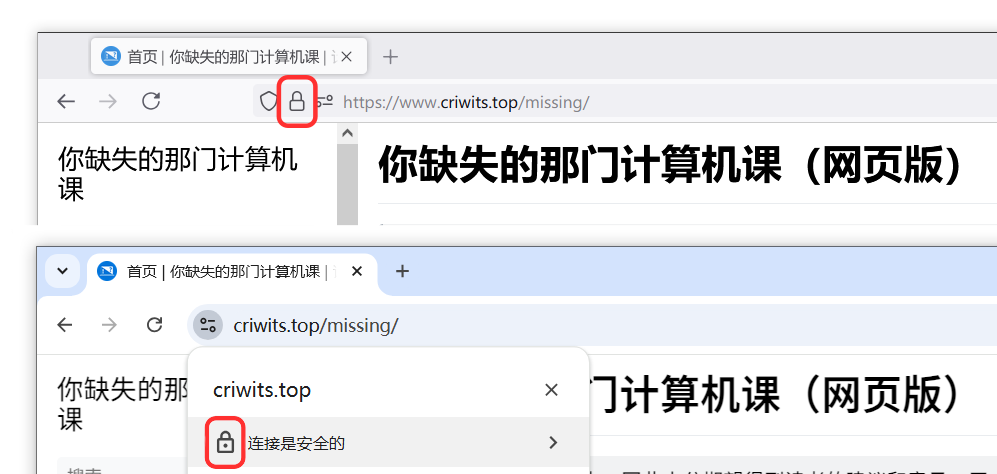
\includegraphics[width=.75\textwidth]{assets/surpass/Lock_signs_in_browsers.png}
  \caption{浏览器地址栏的挂锁图标}
  \label{fig:Lock_signs_in_browsers}
\end{figure}

上图中,上方是 Firefox 浏览器,下方是 Chrome 浏览器。挂锁图标表示网页使用了「HTTPS」传输协议,即「超文本传输安全协议」。这种协议通过多种密码学技术来保护网页和数据。如今,大多数网站都已采用 HTTPS,为我们的数据提供安全保障。下面,就让我们以《你缺计课》网页版为例,看看密码学技术是如何在网络安全中应用的。

\begin{warning}
  \regcolor{如果可能,不要在任何没有启用 HTTPS 的网站上输入任何敏感信息},包括身份信息、登录密码等。我们提到,在互联网上传输的数据,如果不进行加密保护,就可以轻易地被截获和修改。因此,当一个网站没有启用 HTTPS 但是你又在上面输入了这些信息,就可能存在危险。

  一般而言,我们可以通过查看完整网址的开头部分来判断网页是否启用 HTTPS——启用了 HTTPS 的网页,网址以 \MissingTT{https://} 开头,而未启用的则为 \MissingTT{http://} 开头,少了一个 \MissingTT{s}。但是在一些特殊情形下,网址以 \MissingTT{https://} 开头,HTTPS 却可能处于失效状态。好在,大多数浏览器会使用醒目的提示标出没有 HTTPS 的网页,例如被红色斜杠划掉的挂锁、三角警告图标以及【不安全】字样。

  \begin{center}
    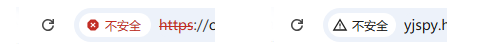
\includegraphics[width=.65\textwidth]{assets/surpass/Non-https.png}
    \captionof{figure}{非 HTTPS 网页}
    \label{fig:Non-https}
  \end{center}

  目前,我国仍然有一些政务、银行网站等由于历史原因未启用 HTTPS。在它们诞生的年代,比较流行的一种做法是在网页内部用自己的方式实现敏感信息的加密,而不使用通用的 HTTPS。还有一些只能通过内网访问的网站,如学校、公司的内部网站,由于无法从外部访问,不太需要 HTTPS 加密来保证安全。作为一些特例,在这些网站上输入信息理论上问题不大,不过在使用它们前,请仔细检查确认你所使用的网站是否为官方网站。
\end{warning}

\subsection{字字皆「机密」——加密与解密}

之前我们已经说了那么多的密码与加密算法,但到现在为止它们都像是空中楼阁——它们到底是怎样应用到实际的呢?现在,是时候看看 HTTPS 背后的密码学了。为了保证传输的超大量网络内容都安全无虞,HTTPS 使用了混合密码——结合对称密码的速度与非对称密码的安全——来加密传输所有内容。

你如果正在电脑上使用 Chrome 浏览器,可以按下 F12,在右上方找到【隐私与安全】(或者【Privacy and Security】)选项卡,就会发现这一句话:

\begin{quoting}
  与此网站的连接已使用 TLS 1.2、包含 P-256 的 ECDHE\_{}ECDSA 和 AES\_{}128\_{}GCM 进行加密和身份验证。
\end{quoting}

\begin{figure}[htb!]
  \centering
  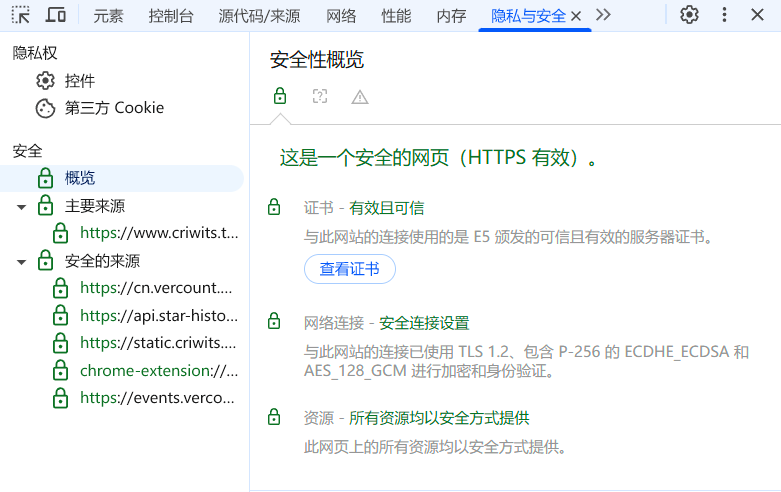
\includegraphics[width=.6\textwidth]{assets/surpass/HTTPS_in_criwits.png}
  \caption{Chrome 显示的加密信息}
  \label{fig:HTTPS_in_criwits}
\end{figure}

这句话告诉了我们藏在《你缺计课》网页版背后的加密算法:

\begin{itemize}
  \item ECDHE 是一种基于椭圆曲线的密钥交换算法,它有点像我们提到的非对称加密算法如 RSA,也有成对的公钥与私钥,不过它专门被用来在通信双方交换后续加密的密钥——也就是接下来提到的 AES 算法的密钥;ECDSA 则是基于椭圆曲线的数字签名算法,关于数字签名的更多内容,请继续阅读本文。
  \item AES\_{}128\_{}GCM 则代表以 128 位为密钥长度的 AES 加密算法。当收到由之前由 ECDHE 传输过来的密钥之后,浏览器就有能力解密通过 AES 加密后传输过来的真正的网页内容,随后送给浏览器渲染并呈现在你眼前。
\end{itemize}

除了 HTTPS 以外,另一个我们身边的直观加密例子是 Windows 系统本身——Windows 使用 AES 加密算法来保护我们硬盘上的数据。在\chapref{cha:user-and-ms-account}一章中我们提到,Windows 提供了一种「设备加密」功能,启动该功能后,硬盘上的所有数据都会被加密存储。这种技术的「真名」叫做 BitLocker,它使用 AES 加密算法来保护硬盘上的数据,而密钥受电脑内部的安全芯片保护。一旦这个安全芯片检测到「情况不对」,就会拒绝提供密钥,从而牢牢地 \CJKsout*{拦住正常的用户} 保护数据的安全。

\begin{note}
  BitLocker 设计有一套复杂的密钥管理系统,因此我们在\chapref{cha:user-and-ms-account}中提到的那个「48 位字符的密钥」并不是实际用于 AES 算法的密钥。实际用于 BitLocker 的 AES 的密钥长度是 128 位或 256 位。
\end{note}

从网络通信,到个人信息,身边无数的例子都在提醒我们:字字皆「机密」,没有密码,信息的安全就无从谈起,我们正常生活的保障也烟消云散。

\subsection{完整才是硬道理——校验和与哈希}

在本书的\chapref{cha:bring-intelligence-to-machines}一章中,我们讲述过过 AI 与人类本质的区别。如果某个攻击者在文章从服务器向我们传输的过程中,蓄意拦截、篡改部分内容,但让其他数据正常发送,让整段文字变成这样(涂黑的是拦截掉的内容,红色是篡改的内容):

% 此段与《AI》的「是敌还是友」一节联动
\begin{quoting}
  {\color{MissingRed}诚}然,「意识」\CJKsout*[thickness=2.5ex, format=\color{black}]{作}为我们人类独有的特质\CJKsout*[thickness=2.5ex, format=\color{black}]{,是这样的「预测机」难以望其项背的}。我们能够\CJKsout*[thickness=2.5ex, format=\color{black}]{在}思考\CJKsout*[thickness=2.5ex, format=\color{black}]{的基础上创新},而 AI {\color{MissingRed}同样}将\CJKsout*[thickness=2.5ex, format=\color{black}]{文字排列组合,}生成\CJKsout*[thickness=2.5ex, format=\color{black}]{一些看似}合理的内容;我们具有复杂的语言和情感,但 AI \CJKsout*[thickness=2.5ex, format=\color{black}]{从未将它们}真正理解,\CJKsout*[thickness=2.5ex, format=\color{black}]{遑论给出}心心相惜\CJKsout*[thickness=2.5ex, format=\color{black}]{的回馈}。更实际一点来说,我们能说着话的同时也顺便唱两句歌,但\CJKsout*[thickness=2.5ex, format=\color{black}]{ AI 还要在各个模型之间切来切去。即使是今天最先进的大语言模型,}错误的回答与偏颇的判断仍屡见不鲜;而人类无穷无尽的想象力、领导力和逻辑能力,是人工智能技术\CJKsout*[thickness=2.5ex, format=\color{black}]{永远}也{\color{MissingRed}能够}完全实现的。
\end{quoting}

整段文字的意思就整整调转了 180 度。这种偷梁换柱、断章取义的风险让我们意识到保护数据的完整性极为重要。

那么,如何保障数据传输的完整性呢?对数据进行加密就是一种重要的方法。在前文我们提到过,今天多数加密算法都可以实现「改变明文中的一小处,整个密文都会变化」——这意味着明文的影响扩散到了整个密文当中。这样,当数据加密传输时,攻击者就很难精确地修改和破坏特定部分的数据了。明文的每一个字都会影响整个密文,反过来更改密文中的每一部分都会影响整体的解密。

不过,仅仅借助加密来保护数据完整性是远远不够的。像 DES、AES 这样的分组加密算法,需要先将完整数据切成固定长度的小块,这使得扩散带来的影响只局限于每一块内部。尽管人们提出了许多解决这一问题的方案,但是「道高一尺,魔高一丈」,精明的攻击者也在不断寻找这些方案的漏洞。为了保护数据的完整性,我们需要打开新思路:在想办法防止数据被破坏之外,我们还应该设计一种能够快速判断数据是否完好的方式。这样,在收到数据之后,只用通过一次检测,我们就能知道数据完好与否了。

我国居民的身份号码就是这种方式一个典型的应用。每个人的身份证上都印有由 18 个数字(或字母)组成的「公民身份号码」,但事实上,第 18 位是由前 17 个数按照下面的算法计算出来的:

\begin{itemize}
  \item 先将第 1 至 17 个数分别乘以下表提供的系数;
    \begin{table}[htb!]
      \centering
      \caption{计算系数表}
      \label{tab:id-check-num-factor}
      \begin{tblr}{
        cells = {halign = c, font = \ttfamily},
        column{1} = {halign = c, fg = white, bg = missing, font = \bfseries},
        column{even} = {MissingSkyBlue},
      }
        \toprule
        序号 & 1 & 2 & 3 & 4 & 5 & 6 & 7 & 8 & 9 & 10 & 11 & 12 & 13 & 14 & 15 & 16 & 17 \\
        系数 & 7 & 9 & 10 & 5 & 8 & 4 & 2 & 1 & 6 & 3 & 7 & 9 & 10 & 5 & 8 & 4 & 2 \\
        \bottomrule
      \end{tblr}
    \end{table}
  \item 然后,将这 17 个乘积相加,再除以 11 求余数;
  \item 查找下表,确定最后一位的值。\footnote{所以,身份号码尾巴的「X」是罗马数字 10,而不是英文 X。}
    \begin{table}[htb!]
      \centering
      \caption{最后一位的对应表}
      \label{tab:id-check-num-lut}
      \begin{tblr}{
        cells = {halign = c, font = \ttfamily},
        column{1} = {halign = c, fg = white, bg = missing, font = \bfseries},
        column{even} = {MissingSkyBlue},
      }
        \toprule
        余数 & 0 & 1 & 2 & 3 & 4 & 5 & 6 & 7 & 8 & 9 & 10 \\
        最后一位 & 1 & 0 & X & 9 & 8 & 7 & 6 & 5 & 4 & 3 & 2 \\
        \bottomrule
      \end{tblr}
    \end{table}
\end{itemize}

这套算法称作 MOD 11-2,定义在国际标准 ISO 7064 中。最终计算出来的值称为「校验码」,它能够用来帮助判别整个号码是否存在错误——假如某人在输入自己身份号码时,不小心写错了其中的几个数,那么最终计算出来的校验码,就很可能与号码最后一位不一致了——当检测到这种不一致时,就可以让系统给出「号码有误」的提示,从而避免后续的麻烦。

\begin{note}
  不妨用自己的身份号码代入上面的算法,计算出来的校验位是否匹配?\CJKsout*{(如果不匹配,说明你算错了或者看错了。)}随机修改其中的一两位再计算呢?
\end{note}

如果我们设计一种类似的算法,给要传输的数据也计算一个「校验码」,并将这个「校验码」与数据本身一同发送——当接收方收到信息后,重新计算一次「校验码」并与之进行比对,不就能保障数据的完整性了吗?不过,由于通信传输的数据通常不只有几个数字那么简短,计算得到的「校验码」自然不像身份号码那样只需要一位数码就能写下,我们将这样的「校验码」称为「校验和」(checksum)。CRC32 是一种常用的校验和算法,输出长度为 32 位,即位于 $0$ 至 $2^{32}-1$ 之间。下面,我们选取了一些字符串作为输入,计算了它们的 CRC32 校验和:

\begin{table}[htb!]
  \centering
  \caption{一些字符串的 CRC32 值}
  \label{tab:some-crc32}
  \begin{tblr}{
    colspec = cccc,
    row{1} = {valign=m, fg = white, bg = missing, font = \bfseries},
    row{even} = {MissingSkyBlue},
    vline{3} = {solid},
  }
    \toprule
    字符串 & CRC32 校验和 & 字符串 & CRC32 校验和 \\
    \midrule
    \MissingTT{Missing} & 1254083771 & \MissingTT{Mis5ing} & 3234525209 \\
    \MissingTT{Missinh} & 1097985814 & \MissingTT{missing} & 2050358017 \\
    \MissingTT{Missin}  & 3616188434 & \MissingTT{Mising}  & 2486458582 \\
    \bottomrule
  \end{tblr}
\end{table}

不难发现,只要输入字符串中有任意一个字符改变或丢失,计算得到的校验和就与原来相去甚远。这说明\regcolor{校验和具有敏感性},对极小的变化有巨大的反应,如此一来,它就能有效地检测出数据是否完整——只要实际校验和与传输的值不一致,就说明数据被破坏。

为了防止攻击者将消息本身和校验和一同篡改,我们可以将校验和与加密结合。对于要发送的数据,我们先计算它的校验和,将数据与校验和拼接在一起一同加密并传输。接收方收到密文后,先将消息解密,再重新计算校验和检验完整性。由于攻击者很难在破坏消息的同时伪造出新的校验和,更难以将伪造的校验和重新进行加密,数据的完整性在这其中便得到了保护。\autoref{fig:Use_checksum_with_encryption} 展示了这一过程。

\begin{figure}[htb!]
  \centering
  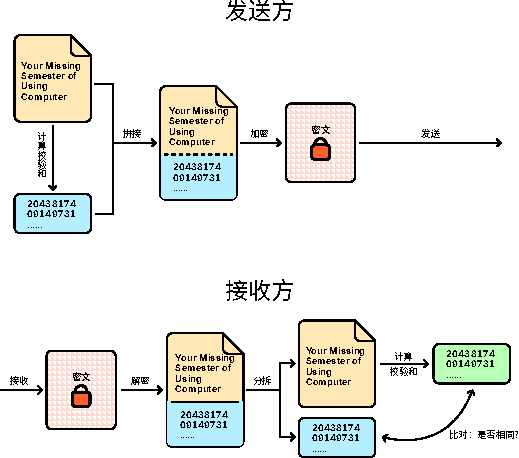
\includegraphics[width=.7\textwidth]{assets/surpass/Use_checksum_with_encryption.pdf}
  \caption{使用校验和与加密算法保障完整性}
  \label{fig:Use_checksum_with_encryption}
\end{figure}

看起来,使用校验和就可以完美地解决「判断数据完好」这一任务了……吗?仍然有个小问题:会不会存在两个数据具有相同的校验和呢?答案是肯定的——还是以身份号码为例,由于校验码一共就 0—9 和 X 总共 11 种情况,你随意在身边找找,就能找到两个人的身份号码有一样的校验码。而在 CRC32 中,校验和亦只有 32 位,一共也只有 $2^{32}=4\,294\,967\,296$ 种情况。由于 CRC32 的运算并不复杂,这让攻击者可以在伪造消息的同时保持校验和不变——如同从 DES 走向 AES 的过程一样,人们需要一种更长、更安全的「校验和」,哈希函数自此登上了历史的舞台。

在密码学中,哈希函数和校验和看起来很像,都能针对任意长度的输入数据计算出一个固定长度的值(称为哈希值),并且极具敏感性。不过,校验和的内部是比较简单的数学运算(例如 CRC32 就基于二进制除法),输出比较短,而哈希函数内部由多次重复而复杂的操作组合而成,输出很长,通常达到上百位。与普通的校验和相比,哈希函数除了具有更强的敏感性之外,还具有很强的\regcolor{单向性}和\regcolor{抗碰撞性}:从哈希值反推输入的难度极高,而找到具有相同哈希值的两个输入也几乎不可能。

过去,常用的哈希函数是 MD5,它的输出长度为 128 位。不过,它已经在 2004 年已经被我国密码学家王小云院士「破解」\footnote{指找到一种高效的算法,能够寻找与给定消息相同哈希值的输入,从而使哈希函数的抗碰撞性不再满足。}。目前常用的被认为安全的哈希函数是 SHA-2 家族,包括 SHA-256、SHA-384 等不同规格,其中又以 SHA-256 最为常用。

在许多软件的下载界面,开发者会在网页上提供一个哈希值(通常使用 MD5 或 SHA-256),这样我们下载软件之后,可以在安装之前自行计算一遍哈希值并与开发者提供的相比对,从而确保我们下载的文件完好无损。\autoref{fig:Hashes_at_download_page} 中,上方为开源音频编辑软件 Audacity 下载页面提供的哈希值,下方则是下载 Go 编程语言的编译器时提供的 SHA-256 值。

\begin{figure}[htb!]
  \centering
  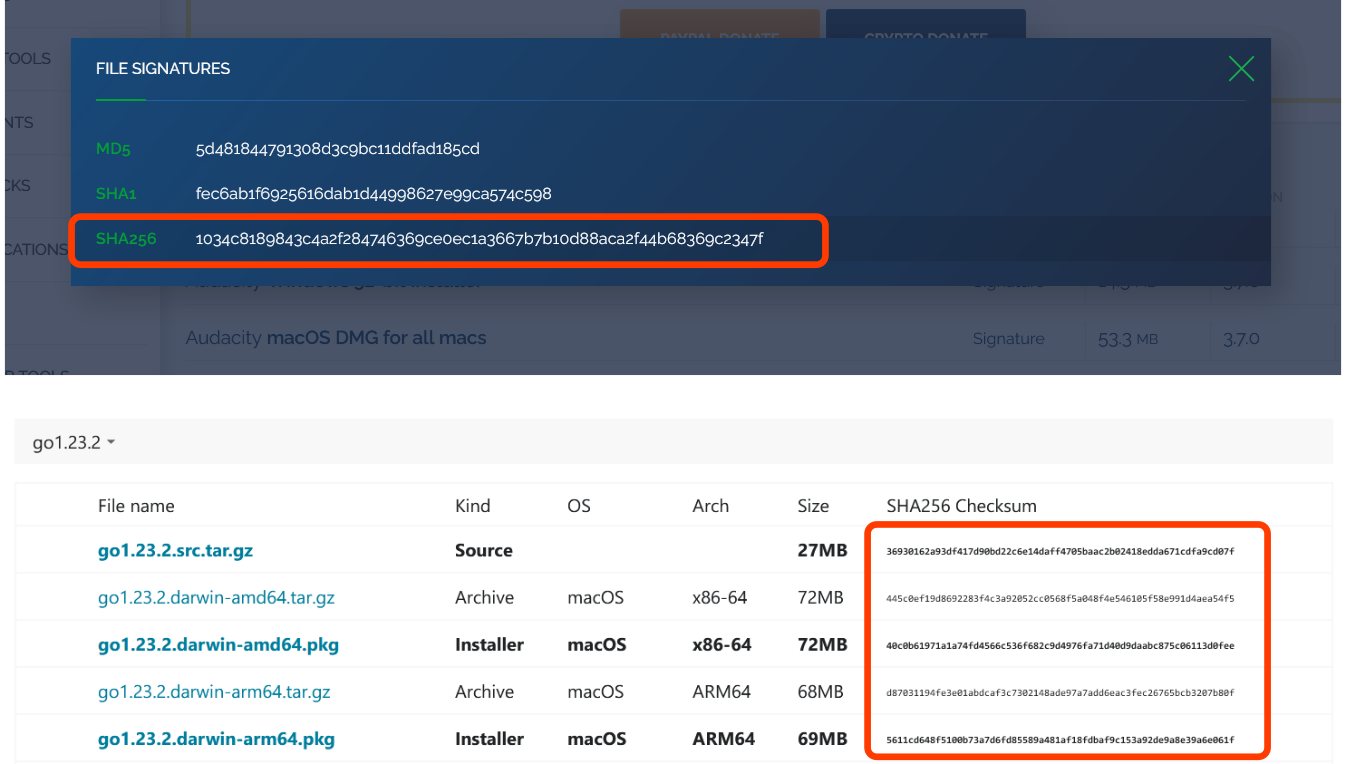
\includegraphics[width=.7\textwidth]{assets/surpass/Hashes_at_download_page.png}
  \caption{下载界面提供的哈希值}
  \label{fig:Hashes_at_download_page}
\end{figure}

而回到你正在阅读的《你缺计课》,我们使用的 HTTPS 技术亦在使用 SHA-256 对数据进行校验,来确保你看到的文字没有在传输过程中遭到修改。如果你正在使用 Firefox 浏览器阅读本网站,不妨点击地址栏前方的挂锁图标,选择【连接安全】→【更多信息】,就能在【技术细节】下方看见:

\begin{quoting}
  连接已加密(\MissingVerb{TLS_ECDHE_ECDSA_WITH_AES_128_GCM_SHA256},128 位密钥,TLS 1.2)
\end{quoting}

其中的 \MissingTT{SHA256} 就是指 SHA-256。

\subsection{铸就「信任」的链条——签名与证书}

现在,距离构建「安全之城」还差最后一块拼图——可认证性。所谓「可认证性」,是让通信另一端的对象的身份可认证。试想一个糟糕的情况:某天你正兴致勃勃地打开《你缺计课》网页版,准备看看我们最新的文章。然而,不怀好意的攻击者直接伪装成我们的服务器,和你交换密钥、加密通信,截获你的所有请求——比起干扰、篡改、破坏已经建立的通信,这回攻击者反客为主,替代我们坐到了你的对面。这个伪造的《你缺计课》网页版看上去和真网站一模一样,不过里面的内容却是……
% \vspace*{-1ex}

\begin{quoting}
  \begin{itemize}
    \item 使用「格式化」功能,就可以轻松清理硬盘垃圾!
    \item AI 即将取代人类,请读者早日购买我们的「被人工智能取代保险」。
    \item 《你缺计课》影响力不断壮大,即将在书店里和各位面世!
    \item 小知识:这四句话中有两句是真的,两句是假的。
  \end{itemize}
\end{quoting}

% \vspace*{-1ex}
在前两小节,我们介绍了如何防止通信被窃密、如何防止传输被破坏,但若不实现通信的可认证性,网上的任何事物我们都无法确认真假。那么,如何才能做到这一点呢?让我们再一次返璞归真,来看一看在赛博世界之外,现实中的人们如何解决这一问题。

\begin{note}
  有一个与「可认证性」相关联的性质,叫做「不可抵赖性」,它指的是:如果我们已经确认某个信息来自某人,那个人就不能再抵赖或否认(声称「我没说过」)。这两者之间有着许多联系,但是它们并不是完全等同的,也并不是说实现一者就会自动实现另一者。
\end{note}

签名是当今社会成本最低而最为常用的认证技术。上小学时,老师会要求我们作业写完要给家长签字,以表示家长真的监督过;或是把我们的考卷带回去家长签字,以代表家长真的看过了试卷\CJKsout*{上的分数}。这「家长签名」正是一种认证,因为小学生往往不太可能模仿出家长的飘逸签名,老师也可以通过对比已有签名的方法将坏孩子「绳之以法」。在这二重保险之下,多数学生就只能选择「乖乖就范」\CJKsout*{而痛失快乐童年}。

除了签名,盖章、按指印等也是常用的认证技术,它们在从日常生活到国家机要的各种场合都有广泛的应用。我们不难发现,这些认证物有一个共同的特点:\regcolor{它们只能由待认证方产生,却可以被任何人检验}——签名只有本人才能签署,经过备案的公章仅有一枚,但是其他人都可以对它们鉴别真伪。这种「只能由……却可以……」的\regcolor{非对称性质},我们在前方介绍非对称密码时亦有提到。因此,仿照非对称加密,我们可以设计一种「赛博签名」。

参照非对称密码的设计,「赛博签名」自然也需要公钥与私钥,其中私钥是用来签名的「笔」,而公钥则是别人验证签名的工具。当\regcolor{我们使用私钥为一些信息签名}时,就相当于生成了一段代表「这些信息由我(私钥所有者)产生」的数据,而\regcolor{其他人可以通过公钥验证这段数据的真假}。由于公钥无法推导出私钥,这保证了其他人可以使用公钥验证签名,却不能伪造出我们的签名。这就是「\regcolor{数字签名}」(digital signature),在后文中我们直接用「\regcolor{签名}」指代它。

我们再回到《你缺计课》网页版的验证问题。有了数字签名,我们的服务器(签名者)就可以用自己手里的私钥给内容签名,将签名与内容一同传输到你的设备。接下来,你的设备(或其他人)可以用服务器的公钥验证签名,也就能确定内容的真实性。这就是「验签」的过程,如\autoref{fig:Signing} 所示。

\begin{figure}[htb!]
  \centering
  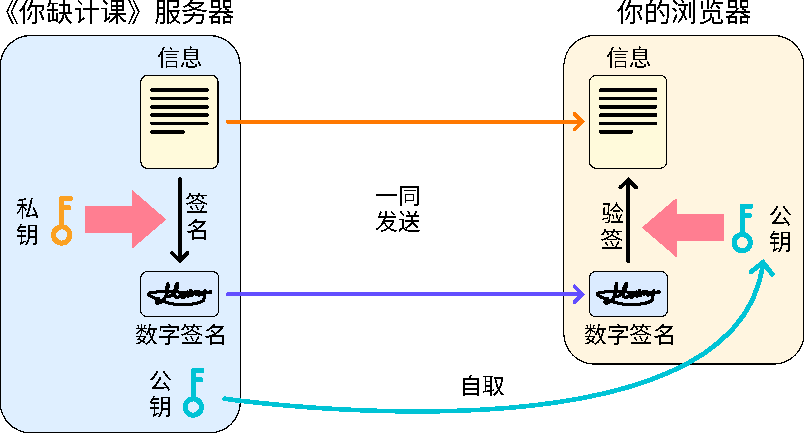
\includegraphics[width=.62\textwidth]{assets/surpass/Signing.pdf}
  \caption{用签名来保证真实性}
  \label{fig:Signing}
\end{figure}

\begin{note}
  和手写签名不同,数字签名与信息内容有关。同一个人给不同信息产生的签名必须不同,不然签名就可以被其他人拿来移花接木。但是,信息内容本身可能很长,为了让签名变得快速、简短,我们又该怎么让签名「和信息相关」呢?(提示:哈希。)请自行思考如何高效签名,并尝试优化上面的示意图。
\end{note}

要将数字签名技术付诸实现,就依然离不开从那些单向陷门函数里寻找灵感。下面列出一些目前常用的签名算法,相信这里有许多你认识的面孔。

\begin{itemize}
  \item RSA 数字签名算法:和 RSA 非对称加密算法一样,基于大数分解困难问题。事实上,RSA 算法身上,签名能力与加密能力相伴而生,二者间可直接无缝转换。不过,尽管数字签名和非对称加密之间有千丝万缕的联系,但是不是所有非对称加密都能像 RSA 一样「阴阳调和」。
  \item DSA 数字签名算法:基于离散对数困难问题,由 ElGammal 所提出(这个名字之前也出现过)。NIST 于 1994 年将 DSA 采用为标准。值得一提的是,DSA 的全称是「Digital Signature Algorithm」(即「数字签名算法」),真是直白\CJKsout*{(其实 DES 和 AES 也是一样的情况)}。
  \item 基于椭圆曲线离散对数困难问题的 ECDSA,以及使用「扭转爱德华兹曲线」(twisted Edwards curves)的变种 EdDSA 等。与前两个签名算法相比,它们所需的密钥长度更短,运算速度更快而不失安全性,因此逐渐取代 RSA 而被广泛使用。
\end{itemize}

现在,问题已经解决了。借助签名技术,这下攻击者就算想伪装成我们,也伪造不出我们的签名——因为私钥牢牢掌握在我们手中。一切都很完美……

……吗?思维敏锐的读者,或许已经发现了这里面的问题:用来验签的公钥,它的真实性如何保证呢?想象一下,如果你是伪造《你缺计课》的攻击者,伪造了网页内容,那伪造一个公钥也就是顺便的事情。也就是说,问题只是从「确认内容的真实性」变成了「确认『用来确认内容真实性的公钥』的真实性」而已。只要攻击者多伪造一步,这一切都形同虚设。我们仿佛向前迈进了许多,但其实只是绕圈走回了原点。

\begin{figure}[htb!]
  \centering
  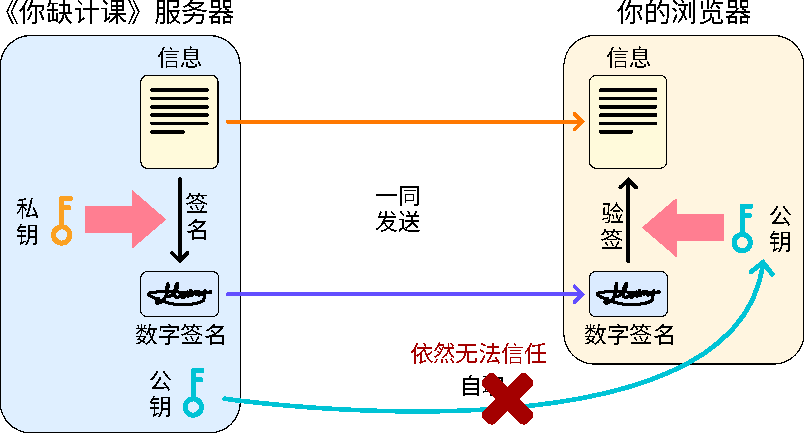
\includegraphics[width=.62\textwidth]{assets/surpass/Signing_invalid.pdf}
  \caption{只靠签名,无法保证真实性}
  \label{fig:Signing_invalid}
\end{figure}

\begin{note}
  当然,我们可以选择再对公钥签一次名,但这样问题就变成了「确认『用来确认「用来确认内容真实性的公钥」的真实性的公钥』的真实性」——\textbf{这不俄罗斯套娃嘛!}我们必须跳出这个循环,寻找一个终结它的方法。
\end{note}

让我们再次返回现实中。现在我们遇到的情况,就如同素未谋面的两人寄信。假设 Hans 和 Windy 互相不认识,现在 Hans 需要给 Windy 写信。尽管 Hans 在信中附上了签名,但由于两人从未见过面,Windy 并不知道对方真实的签名长什么样,所以并不能直接信任这样的签名。这个问题几乎无解,除非\regcolor{遇到一位双方都认识的「信用大户」,并且双方都相信其人品}。有了这样的信用大户,我们就可以请他给 Hans 签署一份这样的证书:

\begin{figure}[htb!]
  \centering
  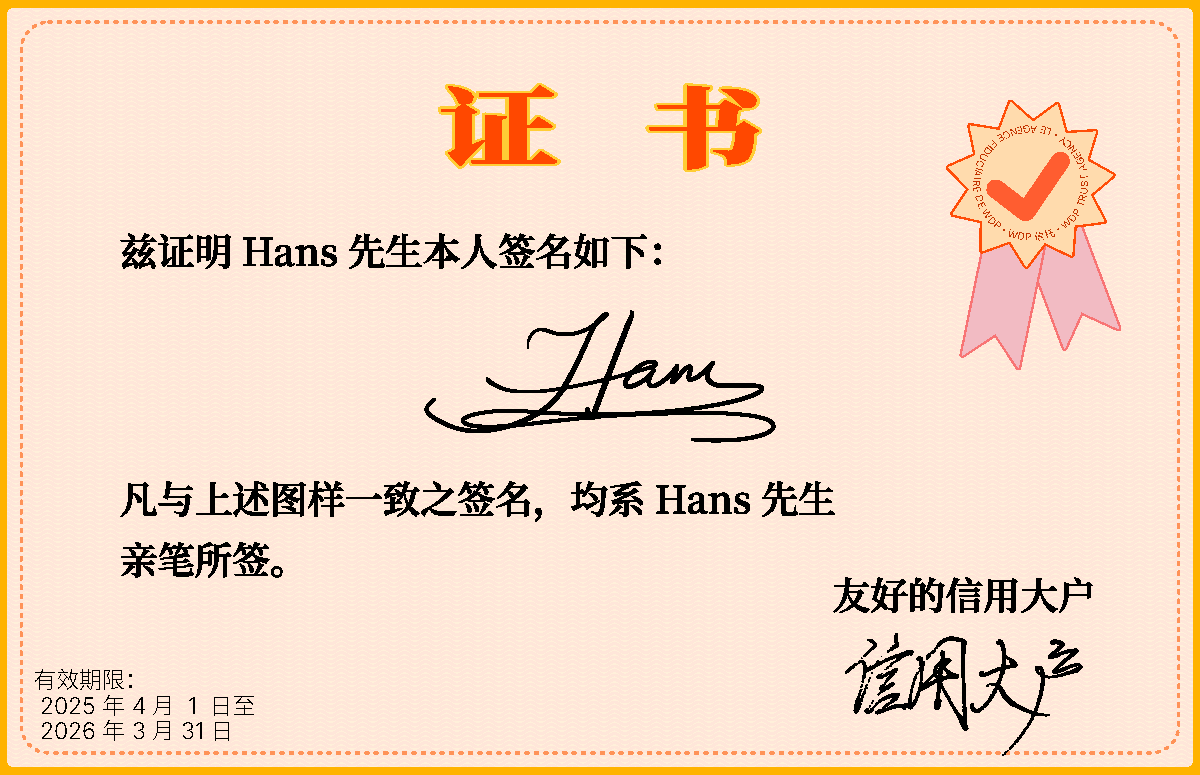
\includegraphics[width=.6\textwidth]{assets/surpass/Certificate.pdf}
  \caption{「证书」}
  \label{fig:Certificate}
\end{figure}

证书由信用大户亲笔签署,提供了一份 Hans 的标准签名样本,从而能验证 Hans 签名的真伪。现在,只要信封里附上这份证书,\regcolor{尽管 Windy 并不直接信任 Hans,但是由于他们都信任这位信用大户,而信用大户为 Hans 担保,双方之间因此构造出了一条「信任链」},实现了可认证性:

\[ \text{Windy} \xrightarrow{\text{信任}} \text{信用大户} \xrightarrow{\text{信任}} \text{Hans} \]

现在,让我们来试试把「证书」的操作应用到数字签名的过程中。现实的证书,证明的是「签名样本」的真实性,而它是用来验签的;但在数字签名中,我们直接使用公钥验签。那么,\regcolor{让信用大户给公钥签个名},不就可以作为一种「数字证书」了吗?

又回到《你缺计课》的例子。如果存在一个你和《你缺计课》都信任的信用大户,我们就可以在向你的浏览器提供内容、签名和公钥的同时,\regcolor{再补充一份「信用大户对我们公钥的签名」作为「证书」}。你的浏览器在收到这个证书后,可以用信用大户的公钥验证它的有效性,进而就验证了我们的公钥的真实性。随后,一切就能像刚刚那套操作一样展开了——借助公钥验签,进而认证安全,就像\autoref{fig:Signing_with_CA}。

\begin{figure}[htb!]
  \centering
  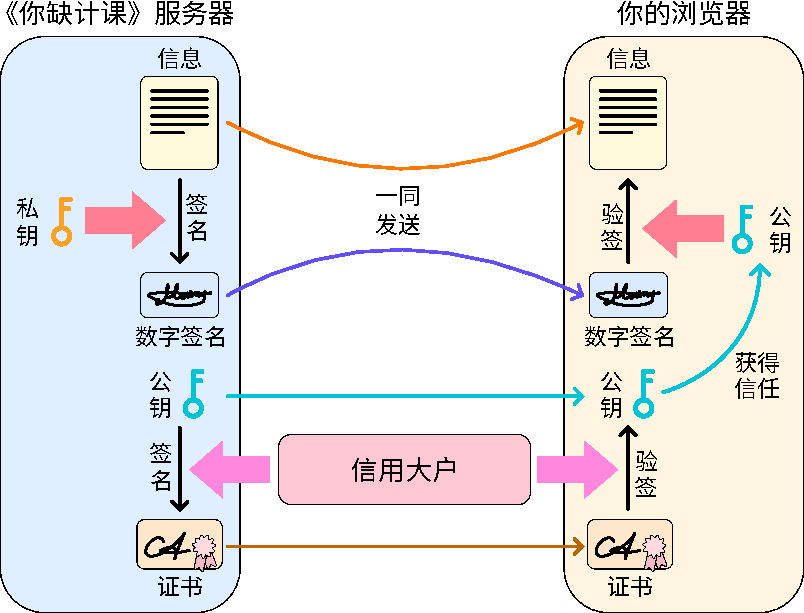
\includegraphics[width=.7\textwidth]{assets/surpass/Signing_with_CA.pdf}
  \caption{让信用大户来确保公钥的真实性}
  \label{fig:Signing_with_CA}
\end{figure}

这就是「数字证书」,本质是信用大户对发信方公钥的签名。在下面的介绍中,我们会直接将数字证书简称为「证书」。

但如果世间所有的通信都需要让双方之间有一位信用大户,就会有两个棘手的问题:第一,信用大户太少,通信数量太多;第二,所有通信者都需要与信用大户有联系,不太现实。那怎么办呢?问题的答案只需四个字:逐级而治。我们只需要请少量几位德高望重的「真·信用大户」,并让世界上的所有人都无条件地信任他们。这几位信用大户不会亲自为所有人签发证书,而是各自给一些「信用小户」签发证书。最后,这些信用小户负责基层工作,基于自身的道德标准,为各种各样的通信方提供证书。

还是考虑《你缺计课》。我们的服务器首先找了一位信用小户来给我们的公钥签发证书。可惜,这位信用小户你的浏览器不认识,所以信用小户还在证书中附了一份他自己的公钥。这个公钥又由一位众所周知的信用大户签名,形成了你能信任的高级证书。当你的浏览器访问《你缺计课》网页版时,服务器会向你提供这一大堆内容:

\begin{enumerate}
  \item 网页内容本身;
  \item 对网页内容的签名;
  \item 我们用于验签的公钥;
  \item \regcolor{信用小户对我们公钥的签名}:这是信用小户给我们签发的证书,称为「终端证书」;
  \item 信用小户用于验签的公钥;
  \item \regcolor{信用大户对信用小户公钥的签名}:这是信用大户给信用小户签发的证书,称为「中间证书」。
\end{enumerate}

你的浏览器只信任信用大户,因此一开始,上面的「六件套」中可以信任的只有最后一项(6 号)。然而,一旦你信任了 6,就可以借助 5 来验证 4 的真实性。验证了 4 的真实性,继而可以验证 2 和 3 的真伪,最终实现对 1 的认证。至此,我们铸就了名为「信任」的链条:

\[ \text{你}\xrightarrow{\text{信任}}\text{信用大户}\xrightarrow{\text{信任}}\text{信用小户}\xrightarrow{\text{信任}}\text{《你缺计课》服务器} \]

\begin{note}
  在现实生活中,不乏这样「逐级信任」的例子。你可以举出一些吗?\CJKsout*{(古时欧洲的封建领主是一个反例,因为他们讲究「附庸的附庸不是我的附庸」。)}
\end{note}

在网络安全的世界里,这些信用大/小户的真身是「\regcolor{证书颁发机构}」(Certificate Authority,\regcolor{简称 CA})。那些德高望重,得到所有人信任的 CA 名为「根 CA」,而实际下到基层,解决群众困难的 CA 则是「中间 CA」。世界上几乎所有需要联网的操作系统,都内置了一份可以无条件信任的「根 CA 列表」,包含:

\begin{itemize}
  \item 所有可信任的根 CA 名单;
  \item 这些根 CA 的公钥。
\end{itemize}

凭借这份列表,整个信任链有了一个可靠的起点。如果你正在使用 Chrome 浏览器,可以点击右上角的【\makebox[.8em]{\raisebox{.6ex}{\rotatebox[origin=c]{90}{...}}}】,选择【设置】,点击【隐私和安全】→【安全】→【管理证书】,再在左侧选择【Chrome 根存储区】。你会看到一个长长的列表,它列出了你的浏览器无条件信任的根 CA。

\begin{figure}[htb!]
  \centering
  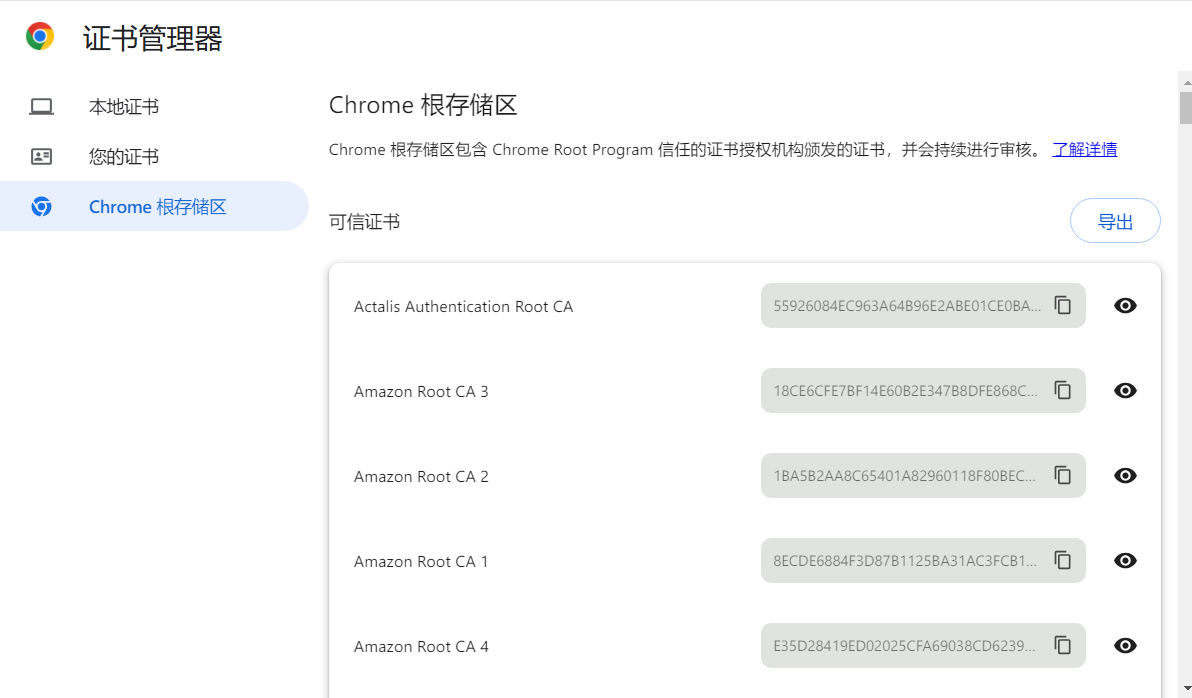
\includegraphics[width=.65\textwidth]{assets/surpass/Chrome_Root_CAs.png}
  \caption{Chrome 信任的根 CA}
  \label{fig:Chrome_Root_CAs}
\end{figure}

而在 Firefox 浏览器上,你可以点击右上角的【≡】,打开【设置】,在左方选择【隐私与安全】,然后下翻找到【证书】一节,点击【查看证书】,你会看到一个类似的列表。

\begin{figure}[htb!]
  \centering
  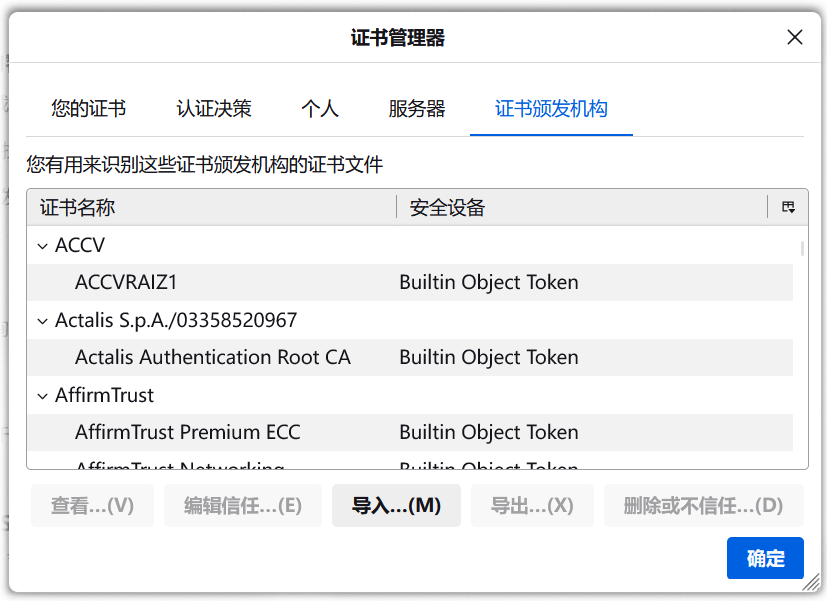
\includegraphics[width=.5\textwidth]{assets/surpass/Firefox_Root_CAs.png}
  \caption{Firefox 信任的根 CA}
  \label{fig:Firefox_Root_CAs}
\end{figure}

借助 CA、证书和签名技术,即使通信双方之间完全陌生,实现可认证的通信也能成为现实。《你缺计课》网页版(实际上是「计算机技术学习札记」全站)拥有一家中间 CA 签发的证书,而这份证书又由一家根 CA 所签名。由于根 CA 位于你浏览器的信任列表中,因此《你缺计课》也能得到信任。

如果有人试图拦截你访问《你缺计课》的流量,并伪造我们的网站,那么这条信任链必然在某处断开。这时,你的浏览器就会检测到问题,并且用显眼的方式警示你「不安全」。在本节开头介绍 HTTPS 时,我们说有时「HTTPS 会失效」,其原因就是信任链的破坏。

\section{迈向多元化的安全}

现在,我们已经在密码学的基础上,构筑了保密性、完整性和可认证性「三位一体」的网络安全之城:加密算法是一切的根源,哈希技术是化繁为简的手段,而签名与证书则带来了「信任的曙光」。各种各样的密码学技术,铸成了我们手中的一把「利剑」,守护着互联网世界的安全。

然而,我们所介绍的这些方面,仅仅是今天网络安全世界的冰山一角。因为,我们只解决了「让信息安全地从一处传到另一处」这件事。无疑,它是维护网络安全的一件头等大事,但实际上,信息从产生开始就面临着安全威胁和挑战:产生信息的设备是否被坏人控制?产生信息的人有没有可能是间谍?整个过程又是否只是设计好的「剧本」,目的只是从我们手中套取有价值的情报?种种问题让我们清楚地认知到,形成多元化、立体化的安全,已经势在必行。

限于本书的篇幅,我们没有办法将这些完全向你展开。幸运的是,在国家、社会和广大人民的共同努力下,今天我们的网安之城正在向着这样的目标稳步前进。上至多部国家级法律的出台,下至公民不断提升的安全意识,再到一口气读完这篇 2 万字长文的你——在充满危机的黑暗世界里,我们共同点燃了希望的火光。

\practice

\begin{enumerate}
  \item 已知偏移量为 5,解密凯撒密码:\MissingTT{Dtzw sfrj nx zspstbs, dtzw kjfy nx nrrtwyfq}。
  \item 诸如 AES 和 DES 这样的分组密码,通过将消息分块进行加密,如果攻击者篡改了密文中的一块,会影响其他块的解密吗?这会造成什么问题?上网搜索「CBC 模式」,看看人们是怎么解决这里的问题的。
  \item 试使用公钥 $(n,e)=(34, 3)$ 加密消息 $m=5$,然后用私钥 $d=11$ 解密它。
  \item 无论是 AES 还是 RSA,都是将一个「数」加密成另一个数,那么如何实现文本的加密呢?(提示:参见\chapref{cha:characters-and-encodings}。)
  \item 假设你需要收集本部门申请补贴员工的材料。现在,你想让大家便携地查阅自己的文件是否提交成功,但为了保护隐私,你不能直接向所有人展示收到的文件列表,你可以怎么做?(提示:文件哈希值。)
  \item 用自己的语言介绍数字签名、数字证书以及它们的应用方式。
  \item 在许多高校,尤其是和国防、航天等国家关键产业联系紧密的高校(如哈尔滨工业大学、北京航空航天大学),「涉密不上网,上网不涉密」的标语在实验室、办公室、教室等地几乎随处可见。想想这是为什么。
\end{enumerate}
